In this chapter we will introduce the notations and concepts we will use in subsequent chapters.


\labelsection{Texts}{subsec:texts}
Text is ubiquitous and the task of automatically processing or classifying text has become more important as the volume of available texts grows daily \cite{Joachims1998}.
While text is arguably the most prominent representation for information for humans, designing algorithms to automatically parse, ``understand" or classify text bear inherent complexities.
Language is a highly complex method to convey information. 
Text often creates its own context, eg. by mentioning some concept in the beginning of a text and only implicitly relating to it at the end. Or by using different words to represent the same concept.
Other difficulties arise due to varying writing styles by different authors.
Another obvious problem is the ambiguous nature of language\cite{Britton1978}, eg. in English the word ``bear" can relate to the animal or the verb.
Often the meaning of a word is defined by its (immediate) context.
Manually defining rules or algorithms to remove the ambiguity of language have been shown to be very laborious if not impossible \cite[p.~11]{Weikum2002}.

These and other difficulties harden the task of processing natural language text significantly \cite{Chowdhury2003,Weikum2002}.
Yet, the task of processing text emerges in important real-world applications.
In text classification, for instance, massive amounts of text make manual assignment of labels virtually impossible, so figuring out automatic approaches to classify text becomes appealing.
Numerous text processing and classification approaches have been proposed in the literature and have shown good accuracy in real-world scenarios.

Since text is most often of non-fixed size, several fixed-size representations have been proposed and employed to enable machine text processing.
One common approach to represent texts is by counting all unique words in a text. The counts of unique words can then be, together with a fixed-size vocabulary, transformed into fixed-size vector representations.
With this approach, some information about the text is omitted, namely the sentence structure, word-order, word-dependency to name just a few \cite{Chowdhury2003}.
So, after transforming a text into this representation, recovering the original text becomes impossible.
That said, while this representation is quite simple and does not capture all information of the text, when using it in the context of text-classification, these representations actually perform very well.
Count-based text representations provide an easy-to-implement baseline and starting point for further improvements.
For example, one extension to this representation does not only gathers the simple one-word counts but also word pairs or consecutive word sequences. These sequences are called $n$-grams, where $n$ stands for the size of such the sequence, eg. $2$-grams consist of 2 words and so on.
In section \ref{sec:evaluation} we will explain these text-based approaches more throughly.

For an recent survey of the history and challenges of natural language processing, see \cite{Chowdhury2003,DeCastilho2014}.

\labelsection{Graphs}{subsec:graphs}
A labeled graph \cite[p.~1]{Bondy1976} is a triple $G = (V, E, \pi)$, where $V$ is the set of vertices or nodes, $E \subseteq V \times V$ are the edges and $\pi: V \to X$ is a labeling function which assigns a label to a given vertex. 
A graph is called undirected when $\forall (v_1, v_2) \in E: (v_2, v_1) \in E$, otherwise it is called directed. 
A graph $G'=(V', E', \pi)$ is called a subgraph of graph $G = (V, E, \pi)$ when $V' \subseteq V$, $E' \subseteq E$ and $\forall (v, v') \in E: v \in V' \land v' \in V' \land (v, v') \in E'$.

The (outgoing) neighbors $n(v)$ of a node $v$ are defined as the set $n(v) = \{v' | (v, v') \in E \}$.

\paragraph{Walks and Paths}
A walk on a graph is a (finite) sequence of edges, $w = (e_1, \cdots, e_n)$ with the constraint that $\forall 0 < i < n: \forall e_i = (v_1, v_2) \in w: \exists v_3: e_{i + 1} = (v_2, v_3)$. The length of the walk is $n$.
The set of all possible walks is denoted $W_G$.
A random walk starting from vertex $v$ is a walk where the first element of walk $w$ is $e = (v, v')$ for some $v'$.

A path is the sequence of the vertices visited on a walk, ie. for the walk $w = ((v_1, v_2), (v_2, v_3), \dots, (v_{n-1}, v_n)$, the path is $(v_1, v_2, v_3, \dots, v_n)$.
The set of all possible paths is denoted $P_G$.

The distance $d_{istance}(v, v')$ between two vertices is defined as the length of the shortest path between them.

\paragraph{Connected components}
A connected component $c$ of a graph is a set of vertices with the constraint $\forall v, v' \in c: \exists p \in P_G: v \in p \land v' \in p$, ie. there exists a path between every vertex in the connected component.
The connected component $c_v$ of a vertex $v$ is the connected component $c$ of a graph where $v \in c$.
The set of all connected components of a graph is $c_{all}(G) = \{ c_v | v \in V \}$. A graph is called connected when there is only one connected component. Only the empty graph has zero connected components.

\paragraph{Degree}
The in-degree $d_{in}$ of a vertex $v \in V$ is $d_{in}(v) = |\{v | (v_1, v_2) \in E \land v_2 = v\}|$.
The out-degree $d_{out}$ is defined analogously as $d_{out}(v) = |\{v | (v_1, v_2) \in E \land v_1 = v\}|$.
The degree of a vertex $v$ is $d(v) = d_{in}(v) + d_{out}(v)$ for directed graphs, and $d(v) = degree_{in}$ for undirected graphs.

\begin{figure}[htb!]
\centering
\begin{tabular}{ll}
symbol &  meaning \\
\midrule
G & Graph \\
$E$ & Set of edges \\
$V$ & Set of vertices \\
$\pi(v)$ & Vertex labeling function \\
$n(v)$ & Neighbours of vertex $v$ \\
$W$ & All possible graph walks on graph $G$ \\
$w$ & Graph walk \\
$P$ & All possible paths on graph $G$ \\
$p$ & Path \\
$d(v)$ & Degree of vertex $v$ \\
$d_{in}(v)$ & In-degree of vertex $v$ \\
$d_{out}(v)$ & Out-degree of vertex $v$ \\
$d_{istance}(v, v')$ & Shortest path length between $v$ and $v'$ \\
$c_{all}(G)$ & Set of all connected components of $G$ \\
$c(v)$ & Connected component of $v$ \\
\end{tabular}
\caption[Notation: Graphs]{Graph notation.}
\end{figure}

\subsection{Concept Map}
A concept map is a directed graph where the nodes are concepts. In our case, the concept maps are automatically constructed from text, yet one can also create them manually.
In our work, concepts are important tokens in the text and consist of one or more words of the underlying text.
An edge between two concepts show that these concepts are related to each other. Edges can have labels also.
For an example of a concept map, see Figure \ref{fig:concept_map}.

\begin{figure}[htb!]
\centering
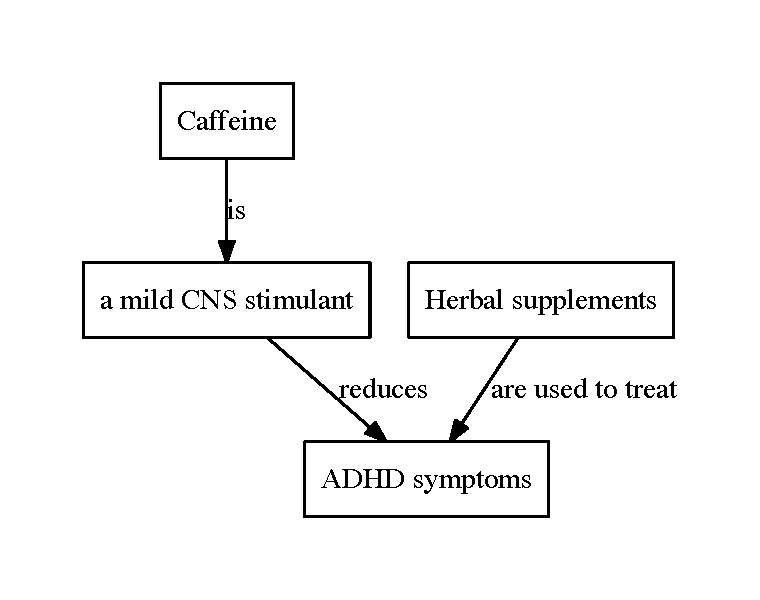
\includegraphics[width=0.5\linewidth]{assets/figures/concept_map.pdf}
\caption[Example: Concept map]{Example of a concept map. The nodes are the concepts. The directed edges connect the concepts to each other and have labels. In this example of a concept map, one could recover sentences from this graph, for example ``Caffeine \textit{is} a mild CNS stimulant". Taken and adapted from: \cite{Falke2017}}
\label{fig:concept_map}
\end{figure}

Concept maps are useful for visualizing concepts and their relation to each other.
They can be used to quickly explore a given topic and immediately see connections between concepts visually.
Through the degree of a concept node, one can also infer the relative importance of that concept in the underlying text.

By combining different texts of the same topic, one can also create a concept map for the whole topic.
In this case, the concepts are not confined to a single text.
The visualization with concept maps of one or more individual texts therefor enables the non-linear exploration of multiple texts of a topic at the same time.
This property makes concept maps interesting in the learning context where visual components become crucial for understanding.
Text, on the other hand, is a linear medium, eg. one often has to read the preceding paragraphs/sections and understand its contents to learn about a new concept.
Extending text, eg. combining several texts of the same topic, also becomes quite laborious since text is inherently linear, so one has to either manually merge the new texts or add side-notes or references to later text passages.
The same task for concept maps can be far easier since one must ``only" find relevant concepts in the texts and their relations to each other. After that the graph can easily constructed.
When the same concept appears in two texts, so the idea, they will be mapped to the same node.
Also, extending a concept map is only a matter of adding new concepts or edges.
One can also augment a node with attributes, eg. add a text that is relevant for this node.
All these properties enable the iterative construction of concept maps by incurring little to no overhead when extending or augmenting concept maps.

Since the concepts in a concept map often contain only a small subset of the text, concept maps also summarize the underlying text.
Only relevant concepts and their relation to each other are captured, making concept maps interesting for (multi-document) text summarization.

Another interesting property is of concept maps with its directed edges is that they can be ``unrolled" into text again, enabling conventional text-processing.
Figure \ref{fig:concept_map_linearization} shows an example of such an unrolled concept map.

\begin{figure}[htb!]
	\centering
	\begin{subfigure}[b]{.48\linewidth}
		\centering
		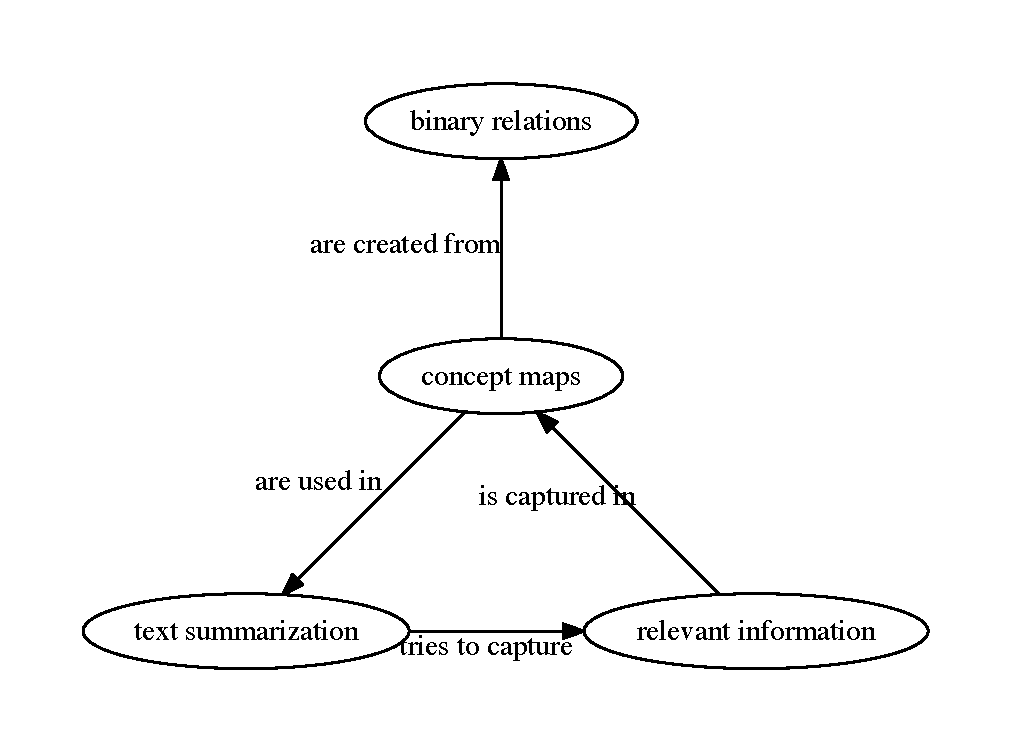
\includegraphics[height=2.2in]{assets/figures/graph_example_linearization.pdf}
		\caption{Concept map}
	\end{subfigure}
	\begin{subfigure}[b]{.48\linewidth}
		\centering
		\noindent\fbox{%
			\parbox{\textwidth}{%
				\textsf{concept maps \enspace\textbf{are used in}\enspace text summarization.
					\\
					concept maps \enspace\textbf{are created from}\enspace binary relations.
					\\
					text summarization \enspace\textbf{tries to capture}\enspace relevant information.
					\\
					relevant information \enspace\textbf{is captured in}\enspace concept maps.
		}}}
		\vspace{0.7in}
		\caption{Extracted sentences}
	\end{subfigure}%
	\caption[Example: Linearized Concept Map]{Example of a concept map with its linearized version.
		The directed edges with their source- and sink vertices get unrolled into sentences.
		Note that there are as many sentences as there are edges in the original concept map.
		Linearizing a concept map in such a way enables conventional text-processing approaches, eg. extracting word counts with \textit{BoW} then classifying with a \textit{SVM}.}
	\label{fig:concept_map_linearization}
\end{figure}

While text is currently arguably the most common medium for information storage, due to the rise of more interactive information mediums, eg. computers, concept maps might become more important in the future.
There are several advantages of concept maps over text, being more structured and visual being to name just a few.
Concept maps therefore have the potential to become a crucial part in the context of information representation and/or learning.

In Chapter \ref{sec:implementation} we introduce the concept map extraction implementation we use and further explain the steps in creating the concept maps automatically from given.

\subsection{Co-Occurrence Graph}
A co-occurrence graph, or graph-of-words, is generated from a text by creating a graph with all the words of the underlying text as nodes.
There is an edge between two nodes if the labels of the source and target node co-occur in the text.
Two words co-occur when the distance between the words in the text is below a given threshold, the window size.
Co-occurrence graphs can have edge weights corresponding to the counts of the co-occurrence of the words in the text.

Figure \ref{fig:cooccurrence_graphs} shows examples of co-occurrence graphs with different windows sizes.

\begin{figure}[htb!]%
    \centering
    \begin{subfigure}[t]{0.32\linewidth}{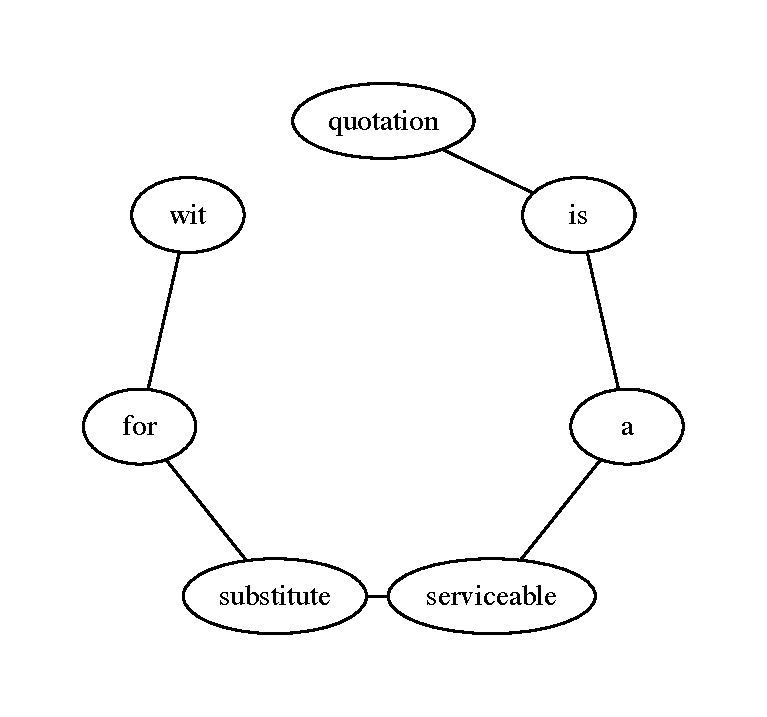
\includegraphics[width=\linewidth]{assets/figures/tmp/cooccurrence_graphs_example/window_size_1.pdf}}%
    \caption{Window size: 1}%
    \end{subfigure}
    \begin{subfigure}[t]{0.32\linewidth}{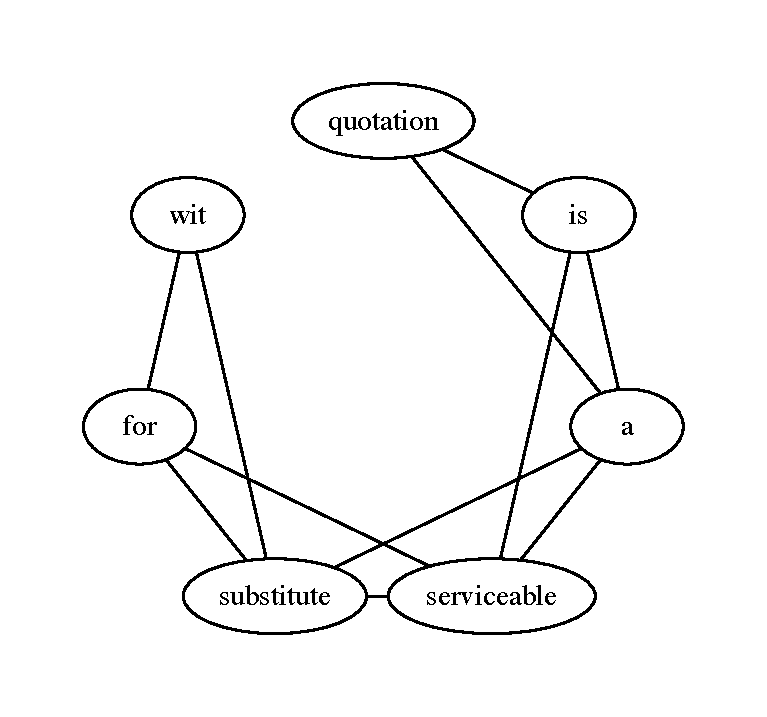
\includegraphics[width=\linewidth]{assets/figures/tmp/cooccurrence_graphs_example/window_size_2.pdf}}%
    \caption{Window size: 2}%
    \end{subfigure}
	\begin{subfigure}[t]{0.32\linewidth}{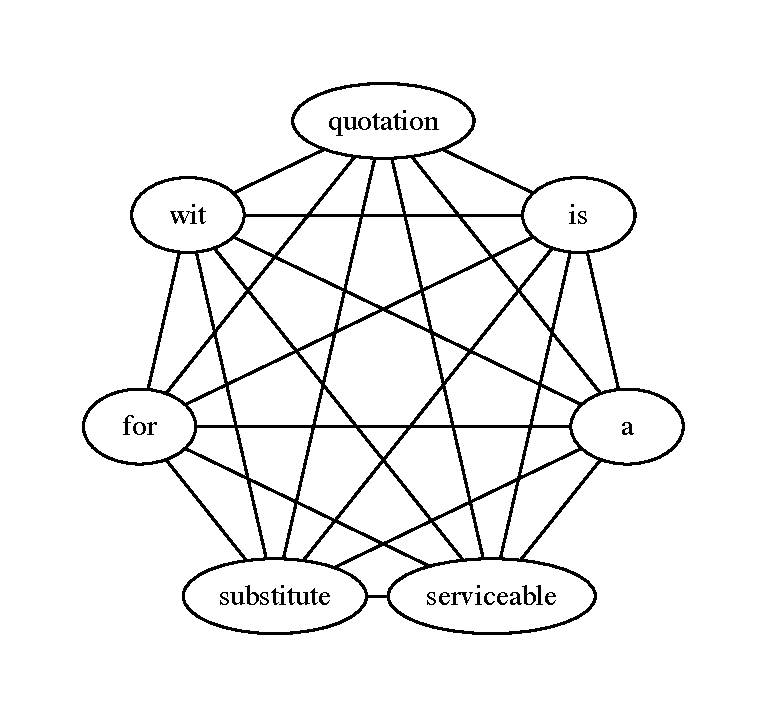
\includegraphics[width=\linewidth]{assets/figures/tmp/cooccurrence_graphs_example/window_size_6.pdf}}%
    \caption{Window size: 6}%
    \end{subfigure}
    \caption[Example: Co-Occurrence Graph]{Example for co-occurrence graphs. Generated from a quote by Jorge Luis Borges\footnote{\url{https://en.wikiquote.org/wiki/Jorge\_Luis\_Borges}}: ``Universal history is the history of a few metaphors". With increasing window size, the number of edges and therefor the connectedness of the co-occurrence graph also increases.}%
    \label{fig:cooccurrence_graphs}%
\end{figure}

\todo{Add example where there co-occurrences also with window size 1}

Since co-occurrence graphs not only contain the words of the underlying text but also their co-occurrence, they capture not only the content of the text but also the relation between words of the text.
Therefor they contain structural information about the text.
But, given a co-occurrence graph, it is not possible to recover the underlying text since all information about word-order or sentence structure is omitted.
That said, one could augment co-occurrence graphs by using directed edges and therefor keep the word-order intact.
Yet, even with this augmentation one can not reconstruct the original text.

Because of their similarity to concept maps, we will use co-occurrence maps as a baseline for the graph classification.
It has to be noted that this comparison is not entirely fair since co-occurrence graphs contain all words of the text and there is only a small loss of information.
The concept maps we extracted on the other hand have a far greater compression factor as we will see, ie. they summarize the content more.
For our comparison, we will also not use the edge weights since concept maps do not have edge weights.


\labelsection{Classification Task}{subsec:classification_task}
Classification using machine learning is the task of automatically assigning classes, or labels, to given datapoints.
Given a dataset $D = \{(x_1, y_1), (x_2, y_2), \ldots, (x_n, y_n) \} \subseteq X \times Y$ of $n$ items where $(x_i, y_i)$ are dataset instances, the supervised single-label classification task is to create a classifier which automatically predicts a label $y' \in Y$ for a given $x \in X$.
The labels $Y$ of dataset $D$ are denoted with $Y_D = (y_1, y_2, \ldots, y_n )$, the predicted labels are denoted as $Y'_D = (y'_1, y'_2, \ldots, y'_n )$.
When the number of classes $|Y| = 2$, the classification task is called binary classification. For $|Y| > 2$ the task falls into the multi-class classification domain.
In this work we will restrict ourself to single-label classification, in contrast to the multi-label classification task where each document can have one or more labels attached instead of only one per document.

In Figure \ref{table:classification_notation} we summarize the classification notation.
Our notation is similar to the notation used in \cite[p.~11]{Bishop2006}.

\begin{table}[htb!]
	\centering
	\begin{tabular}{lll}
		& Notation & Definition \\
		\toprule
		Datapoint & $x$ & $x \in X$
		\\
		Label & $y$ & $y \in Y$
		\\
		Real and predicted label of $x_i$ & $y_i$, $y'_i$ &  $y_i, y'_i \in Y$
		\\
		Instance & $d_i$ & $(x_i, y_i) \in X \times Y$
		\\
		Dataset & $D$ & $\{(x_1, y_1), \ldots, (x_n, y_n) \} \subseteq X \times Y$ 
	\end{tabular}
	\caption[Notation: Classification]{Classification notation.}\label{table:classification_notation}
\end{table}

To automatically assign the labels in a supervised way, generally a learning algorithm is used to train a classifier by providing it datapoints and its labels.
The classifier algorithm then, internally, creates a model of the data and often optimizes internal parameters to fit the data.
During prediction, that is when wanting to automatically assign a label to a (new) datapoint $x_i$, the new datapoint is fed into the classifier which in turn returns the predicted label, $y'_i$.

\labelsubsection{Classifiers}{subsec:classifiers}
In this work, we will mostly use a classification algorithm called \textit{Support Vector Machine} \cite{Cortes1995}, or \textit{SVM}.
The SVM has shown to be robust in its performance \cite{Joachims1998}, having not to deal with local optima as in neural networks or other machine learning algorithms.
The SVM also exhibits state-of-the art performance on several tasks and is the go-to classification algorithm in a great number of previous works in the field \cite{Joachims1998, Vitale2012, Neuhaus2006a,Kriege2012, Koronacki2008}.

For an more throughout explanation of the SVM and its advantages especially for the text classification task, please see \cite{Joachims1998}.
We will also further explain the SVM and its parameters in Section \ref{subsec:cross_validation_and_model_selection}.

\labelsubsection{Performance Metrics}{subsec:classification_metrics}
The performance or score of a trained classifier is evaluated by comparing the labels it predicts, $y'_i$,  for datapoints $x_i$ with the real label $y_i$ in the dataset.
There are several metrics for evaluating the performance of a classifier.
The classification metrics we use in this work are summarized in Figure \ref{fig:classification_metrics}.
For an extensive overview of classification metrics, see \cite{Forman2003}.
In this work, we will use the term classification performance synonymously with classification score, unless otherwise stated.
On the other hand, we will refer to the complexity or run-time of a classification algorithm by the classification run-time.

\begin{figure}[htb!]
	\centering
	\renewcommand*{\arraystretch}{1.7}
	\begin{tabular}{llll}
		& Notation & Definition & \\
		\toprule
		True positives of $y$ &
		$TP_y$ &
		$\displaystyle |\{i | y'_i = y, y'_i = y_i \}|$ &
		\\
		False positives of $y$ &
		$FP_y$ &
		$\displaystyle |\{i | y'_i = y, y_i \neq y \}|$ &
		\\
		True negatives of $y$ &
		$TN_y$ &
		$\displaystyle |\{i | y'_i \neq y, y_i \neq y\}|$ &
		\\
		False negatives of $y$ &
		$FN_y$ &
		$\displaystyle |\{i | y'_i \neq y, y_i = y\}|$ &
		\\[1ex]
		\midrule{}%
		\\[-2ex]
		Accuracy &
		$A$ &
		$\displaystyle \frac{\sum\nolimits_{y \in Y} TP_y}{|D|}$ &
		\\[3ex]
		Precision of $y$ &
		$Pr_y$ &
		$\displaystyle \frac{TP_y}{TP_y + FP_y} $ &
		$Pr_{\text{macro}} = \displaystyle \frac{\sum\nolimits_{y \in Y} Pr_y}{|Y|}$
		\\[3ex]
		Recall of $y$ &
		$R_y$ &
		$\displaystyle \frac{TP_y}{TP_y + FN_y}$ &
		$R_{\text{macro}} = \displaystyle \frac{\sum\nolimits_{y \in Y} R_y}{|Y|}$
		\\[3ex]
		F1 score of $y$ &
		$F1_y$ &
		$\displaystyle 2 \cdot \frac{Pr_y \cdot R_y}{Pr_y + R_y}$ &
		$F1_{\text{macro}} = \displaystyle \frac{\sum\nolimits_{y \in Y} F1_y}{|Y|}$
		\\
	\end{tabular}
	\caption[Notation: Classification metrics]{Classification performance metric notation. As performance metrics, we will us accuracy, macro precision, macro recall and the macro F1 score. The macro version of a metric takes into account how many elements there are in each class which is helpful for skewed datasets, ie. where the number of instances per label is not distributed uniformly per label.}\label{fig:classification_metrics}
\end{figure}


\labelsection{Kernels}{subsec:kernel}
In most cases, texts and graphs are not of fixed size.
However, most classification algorithms operate on fixed size vectors.
Fortunately, there are several approaches to overcome this problem.
One of the approaches to classify non-fixed size objects are so-called kernels.

A kernel is a function $k$ which returns a measure of similarity between two objects:
\begin{equation*}
k: X \times X \rightarrow \mathbb{Q}
\end{equation*}

A kernel function has to be \cite{Kriege2012}:
\begin{itemize}
    \item{\textit{symmetric}: $k(x, x') = k(x', x)$}
    \item{\textit{non-negative definite}: $\forall x, x': k(x, x') \geq 0$}
\end{itemize}

An interesting property of kernels is that they can be combined easily with symmetric operations \cite[p.~296]{Bishop2006}, eg. by adding or multiplicating the results of two kernel functions, $k_1$ and $k_2$:
\begin{equation*}
k_{combined}(x, x') = k_1(x, x') \cdot k_2(x, x')
\end{equation*}

One can easily confirm that, when $k_1$ and $k_2$ are valid kernels, $k_{\mathrm{combined}}$ is also a valid kernel.
This property enables composite kernels to capture multiple means of similarity in one metric.

For example, a simple kernel on two numbers (or vectors) is $k(x, x') = | x \cdot x' |$, where $| \cdot |$ is the absolute value (or a norm).
Another example of a kernel between strings is $k(s, s') = \delta(s = s')$, where $\delta(\cdot)$ is the Kronecker delta. This kernel returns 1 if the two given strings are the same, and 0 if they are different.
Note that both these kernels are indeed valid.
That said, when using kernels in the real world, one can also use non-valid kernels, ie. kernels which are non-symmetric and/or return negative numbers. While such ``kernel" are not strictly valid, they can nevertheless perform good in real-world applications, even better than valid kernels.

Kernels can be used in kernel methods for classification and other tasks.
Prominent examples of kernel methods include the \textit{SVM}, kernelized \textit{Principal Component Analysis} and \textit{Gaussian Processes}.
In Section \ref{sec:kernel_method_and_kernel_trick}, we further explain kernel methods.

For a subset of kernels, one can also create explicit feature vectors, or feature maps, for a given object. In this case, the kernel can be rewritten as an inner product on two fixed-size vectors:

\begin{equation*}
    k(X, X') = \langle \phi(X), \phi(X') \rangle
\end{equation*}

Here, $\phi(X)$ returns a fixed-size vector representation of the object $X$ and is the main part of the kernel.
This $\phi(X)$ can then be used in all vector-based classification algorithms, not only kernel methods.
An example for such a kernel is the string kernel which counts the number of occurrences of words in a given text, then creates a vector representation by giving each word an index in the vector and setting this index to the number of occurrences of that word. The inner product of two of these vector representations then create a kernel.

\paragraph{Gram matrix}
A gram matrix, or kernel matrix, for a given kernel is a matrix $A$ for a set of objects, $D = (x_1, x_2, \ldots, x_n)$ where the entries are the pairwise similarities between all these objects in the dataset:
\begin{equation*}
A_{i,j} = k(x_i, x_j)
\end{equation*}
So, the entry in the $i$-th row and $j$-th column signifies the similarity of $x_i$ and $x_j$ under the given kernel.

When the explicit feature map $\phi(x)$ for each $x$ is given, one can also construct the gram matrix by vertically stacking these feature vectors into a matrix $M_{\phi}$ and calculating the product on the transpose
\begin{equation*}
A = M_{\phi} M_{\phi}^T
\end{equation*}
The gram matrix is symmetric by definition since the underlying kernel is also symmetric, ie. $A_{i,j} = A_{j, i}$.

\labelsubsection{Kernel Methods and Kernel trick}{sec:kernel_method_and_kernel_trick}
We have seen that a kernel can be used to calculate a measure of similarity between two objects, eg. graphs.
Some kernels can be expressed as an inner product $k(X, X') = \langle \phi(X), \phi(X') \rangle$ on two (implicit) vector representations of the objects $X$ and $X'$.
In this case, the vector representations $\phi(X)$ can be used in conventional classification algorithms.
Yet, calculating these representations is not always possible or feasible since the dimension of such a representation is quite high or even infinite, making the calculation unfeasible.
There is another approach for classification and other tasks, the aforementioned kernel methods.
Kernel methods \cite[p.~291]{Bishop2006} operate directly with the kernel and do not use the explicit feature representations $\phi(X)$.
Instead, kernel methods use the similarities $k(X, X')$ directly.
This feature also enables kernel methods to operate on arbitrary objects, given that there exists a kernel operating on these objects.

One popular example for a kernel method is the Support Vector Machine, or SVM.
The SVM is able to use both vector representations of elements in the dataset or the pairwise similarities, the gram matrix, between them.
Some SVM implementations also allow to define the kernel directly, so the gram matrix does not have to be provided.
At training time, the gram matrix $A$ of all objects in the training set, $D_{train} = \{X_1, X_2, \ldots, X_n\}$, is calculated.
This gram matrix $A$ and the corresponding classes then get fed into the SVM which fits its coefficients to them.
After training, to predict the label for a given instance $X_{test}$, the pairwise similarities of $X_{test}$ and all training examples, $\{X_1, X_2, \ldots, X_n\}$, are calculated, resulting in a vector $v = (k(X_{test}, X_1), k(X_{test}, X_2), \ldots, k(X_{test}, X_n))$.
The vector $v$ contains the similarities of $X_{test}$ to all training instances.
This vector $v$ is then fed into the SVM which predicts the label for $X_{test}$.
Note that this kernel method approach does not use explicit feature maps of the instances, only their pairwise similarities.
This feature of not needing to calculate the explicit feature map $\phi$ is called \textit{kernel trick} \cite[p.~292]{Bishop2006}.
The kernel trick also enables linear algorithms, such as the un-kernelized \textit{SVM}, to solve non-linear problems, since the kernel can operate in higher-dimensional spaces	.
The kernel trick can be applied to any algorithm where the core of the algorithm uses vector representations to calculate an inner product. These inner products on the vectors can be replaced with kernels, resulting in a kernelized version of the algorithm \cite{Wu}.
Apart from the kernelized \textit{SVM}, the class of kernel methods also includes kernelized \textit{Principal Components Analysis} \cite{Scholkopf1998}, kernelized \textit{k-Means} \cite{Jain2010}, \textit{Gaussian Processes} \cite[p.~303]{Bishop2006} and others.

In our work, we will use both the kernelized version of the \textit{SVM}, ie. learning with the gram matrix, as well as the version using explicit feature maps $\phi$.

\labelsubsection{Graph Kernels}{subsec:graph_kernels}
A graph kernel simply is a kernel that operates on graphs.
Graph kernels that measure the similarity of two graphs are related to the isomorphism test \cite[p.~4]{Bondy1976} between two graphs.
The (structural) graph isomorphism test returns whether two graphs are structurally the same.
In this test, the labels of the vertices and edges are ignored. Otherwise the task would be far easier since one could simply compare the labels and edges of the graphs - when they are both exactly the same, the graphs are the same \cite[p.~4]{Bondy1976}.
Instead, in the graph isomorphism test one has to find two mappings: one bijective mapping $\psi_{V}: V_1 \mapsto V_2$ from the vertices of the first graph to the vertices of the second graph and another bijective mapping $\psi_{E}: E_1 \mapsto E_2$ with the constraint:

\begin{equation*}
    \forall e = (v_s, v_t) \in E_1:
    \exists e' = (v'_s, v'_t) \in E_2:
    \psi_{E}(e) = e'
    \Rightarrow
    \psi_{V}(v_s) = v'_s
    \land
    \psi_{V}(v_t) = v'_t
\end{equation*}

If such a mapping exists, the two graphs are called isomorphic.
While the complexity of the graph isomorphism test is not known yet, it is suspected to lie in P or it may also be NP-complete \cite{Hido2009,Kulharia2008}.
 
One could use the graph isomorphism test, or a variant thereof, to create a graph kernel $k_{isomorphism}$ by returning 1 if the two graphs are isomorphic and 0 otherwise.
Yet, as we noted before, the runtime of the graph isomorphism test is high and also, in the presented version, does not take edge or node labels into account.
We will see other examples of graph kernels in the next paragraphs.
Note that each graph kernel has different strengths and weaknesses, often being subject to a trade-off between accuracy versus compute time.
So, when choosing a suitable kernel, the importance of each aspect of the graphs, eg. labels or structure, has to be assessed and the kernel constructed or chosen accordingly.

\paragraph{Graph Kernel Categories}
Several graph kernels have been proposed in the literature.
Categories of graph kernels include kernels based on shortest-paths \cite{Hermansson2015, Borgwardt2005, Nikolentzos2017b}, random-walks \cite{Neuhaus2006a} and subtree patterns \cite{Shervashidze2009,Douglas2011,Kersting2013}, to name just a few.

A great number of graph kernels have in common that they first create a decomposition of the graph into sub-structures, for example into subtrees, and then count the occurrences of these sub-structures in the graphs.
The kernels of this kind are sometimes called R-Convolution graph kernels \cite{Namomsa1965a}.
In the next section, we introduce some examples of graph kernels to get a feeling for the possibilities and trade-offs different approaches have.
As mentioned before, any set of valid kernels can be combined easily to form a composite kernel \cite[p.~296]{Bishop2006}.
So, any of the algorithms we will introduce in the next section can be combined and extended using other kernels.
As we will also see in this next section, graph kernels can be quite diverse and capture different information of the objects they are operating on.
The scope of a graph kernel can therefor also vary widely from only capturing narrow aspects of the graph to actually incorporating the complete graph structure and content.

For a more detailed overview on graph kernels, \cite{Gartner2003a} contains a survey of current graph kernel approaches.

\subsection{Examples}
\paragraph{Simple Equality Graph Kernel}
This graph kernel simply compares the nodes and edges of the two graphs and returns whether they are exactly the same:
\begin{equation*}
    k(G_1, G_2) = \delta(V_{G_1} = V_{G_2}) \cdot \delta(E_{G_1} = E_{G_2})
\end{equation*}
This kernel takes both structure and content of the graphs into account. Note that there is no partial similarity. The co-domain of $k$ is $\{0, 1\}$, returning 1 when the graphs are exactly the same and 0 otherwise.
While this is an exact, simple and fast algorithm, in most cases it is not of great use since it depends on exact matches.

\paragraph{Simple Non-Structural Graph Kernel}
Following is an example of a simple kernel which actually discards all structural information about the graph. This graph kernel only operates on the labels of the vertices:
\begin{equation*}
k_{\mathrm{common\_label}}(G_1, G_2) = | l(G_1) \cap l(G_2) |
\end{equation*}
where $l(G)$ returns the set of labels for graph $G$.
Therefor, this graph kernel counts the number of common labels of the two graphs. Under this kernel, two graphs are the same when they have the same node labels, completely ignoring the edges.
While this kernel only compares vertex labels, edge labels could quite easily be added to the kernel definition.

An extension to this graph kernel is using the Jaccard coefficient instead of simply counting the common node labels:
\begin{equation*}
k_{\mathrm{common\_label\_jaccard}}(G_1, G_2) = \frac{| l(G_1) \cap l(G_2) |}{| l(G_1) \cup l(G_2) |}
\end{equation*}
This extension normalizes the function and confines the codomain of $k$ to $[0, 1]$.

\paragraph{Simple Structure-Only Graph Kernel}
An example for a graph kernel which only operates on the structure of the graph, is the following:
\begin{equation*}
k_{\mathrm{simple\_structure}}(G_1, G_2) = \langle \phi(G_1), \phi(G_1) \rangle
\end{equation*}
with $\phi(G) = (n_{\mathrm{triangle}}(G), n_{\mathrm{rectangle}}(G))^T$. Here, $n_{\mathrm{triangle}}$ is the number of the triangle subgraphs in $G$ and $n_{\mathrm{rectangle}}$ the number of rectangle subgraphs in $G$.
This graph kernel is an example of a kernel where the explicit feature map $\phi(G)$ can be computed directly and completely independent of other graphs.
It is also an example for a R-convolution kernel.

The graphlet kernel \cite{Shervashidze2009a} is quite similar to this example kernel $k_{\mathrm{simple\_structure}}$: instead of only counting the number of triangle and rectangle subgraphs, the graphlet graph kernel counts so-called graphlets \cite{Shervashidze2009a}.

\paragraph{Random Walk Graph Kernel}
This kernel does random walks on both graphs and returns the number of matching random walks between the two graphs:
\begin{equation*}
    k(G_1, G_2) = |r(G_1, n, l) \cap r(G_2, n, l)|
\end{equation*}
where $r(G, n, l)$ returns a set of $n$ random walks of length $l$ on graph $G$.
This graph kernel takes both structure and content into account.

\paragraph{Weisfeiler-Lehman Graph Kernel}
The Weisfeiler-Lehman graph kernel is also a kernel that works by counting common sub-structures on two graphs.
Here, the sub-structures are subtrees starting from each vertex.
In each iteration $i$ with $0 < i < h$ for a given number of iterations $h$ , or until convergence, the WL graph kernel relabels the vertices of the two given graphs.
This relabeling is also called recoloring or color refinement.

The WL graph kernel relabels a vertex $v$ by concatenating two components:
\begin{enumerate}
    \item{the current label of the vertex: $\pi_{i-1}(v)$}
    \item{the sorted labels of the neighborhood: $\{ \pi_{i-1}(v') | v' \in n(v) \}$}
\end{enumerate}
where $\pi_{i}$ is the labeling function for iteration $i$ with $\pi_0 = \pi$.
The resulting new label of $v$ is the sequence $(\pi_{i-1}(v), \pi_{i-1}(v_{neighbour,1}), \dots , \pi_{i-1}(v_{neighbour,n}))$.
After the iteration, a new labeling function is created accordingly: $\pi_i(v)$ now returns to the new label of $v$.
So, for each iteration, a node gets the same label as another node if they have the same label and neighborhood.
For the first iteration, the labels of a node consist of the immediate neighborhood.
In the next iteration, the label of a node than encodes the neighborhood of the neighborhood, and so on.
The Weisfeiler-Lehman graph kernel is said to have converged in iteration $h = i$ when the number of used labels does not increase in the next iteration, so
\begin{equation*}
\max(\{x | x = \pi_{i}(v), v \in V\}) = \max(\{x | x = \pi_{i  + 1}(v), v \in V\})
\end{equation*}

The Weisfeiler-Lehman graph kernel has been shown to achieve state-of-the-art performance on several datasets and applications.
It takes into account both content and structure, while also performing good in terms of compute-time.

The runtime complexity of the Weisfeiler-Lehman algorithm varies with different extensions.
Reported complexities of the WL algorithm range from (1) $\mathcal{O}(hm)$ in \cite{Shervashidze2009} where $h$ is the number of iterations and $m$ stands for the number of edges in a graph and (2) the quasi-linear $\mathcal{O}((m + n) \log(n))$ in \cite{Kersting2013} where $n$ stands for the number of edges.

It has to be noted that the Weisfeiler-Lehman does not use edge labels by default, but can be extended to do so.
There are also several other extensions to the Weisfeiler-Lehman kernel in the literature.
One example of such an extension reduces the space requirement of the algorithm by ``compressing" the labels after each iterations, ie. by giving each composite label a unique and shorter label.

In Figure \ref{fig:wl_example} we show an example of one WL iteration with label compression.

In this work we will use a variant of the WL graph kernel called \textit{fast\_wl} which was introduced in \cite{Kersting2013}.
This variant improves the run-time of the plain Weisfeiler-Lehman kernel by cleverly creating a hash of the neighborhood to create the new coloring for the graph, resulting in the aforementioned $\mathcal{O}((m + n) \log(n))$ complexity.
The results for this \textit{fast\_wl} variant are exactly the same as with the plain WL kernel, yet the calculation of the new labels is significantly faster.
Our implementation also uses label compression, explained in Figure \ref{fig:wl_example}, to further speed up the calculation and assigning integer indices to the new labels, therefore enabling the creation of explicit feature maps $\phi(G)$.

\begin{figure}[htb!]
  \centering
  \begin{subfigure}[t]{0.49\linewidth}
  {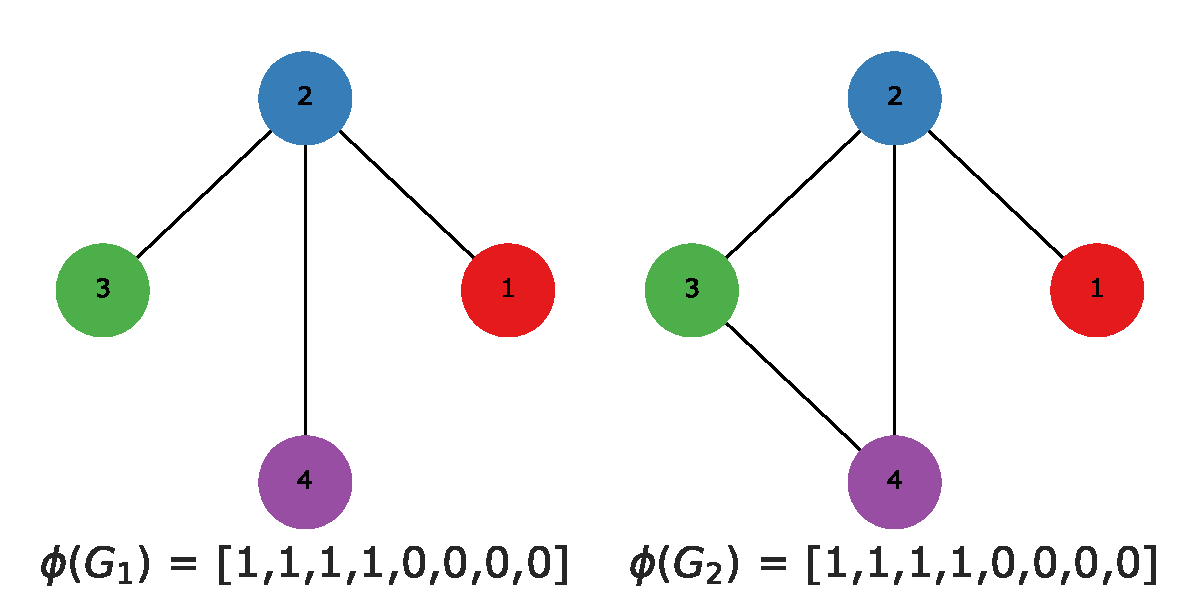
\includegraphics[width=\linewidth]{assets/figures/wl_examples/wl_iteration_0.pdf}\label{fig:wl_example_0}}
  \caption{Initial graphs}
  \end{subfigure}
  \begin{subfigure}[t]{0.49\linewidth}
  {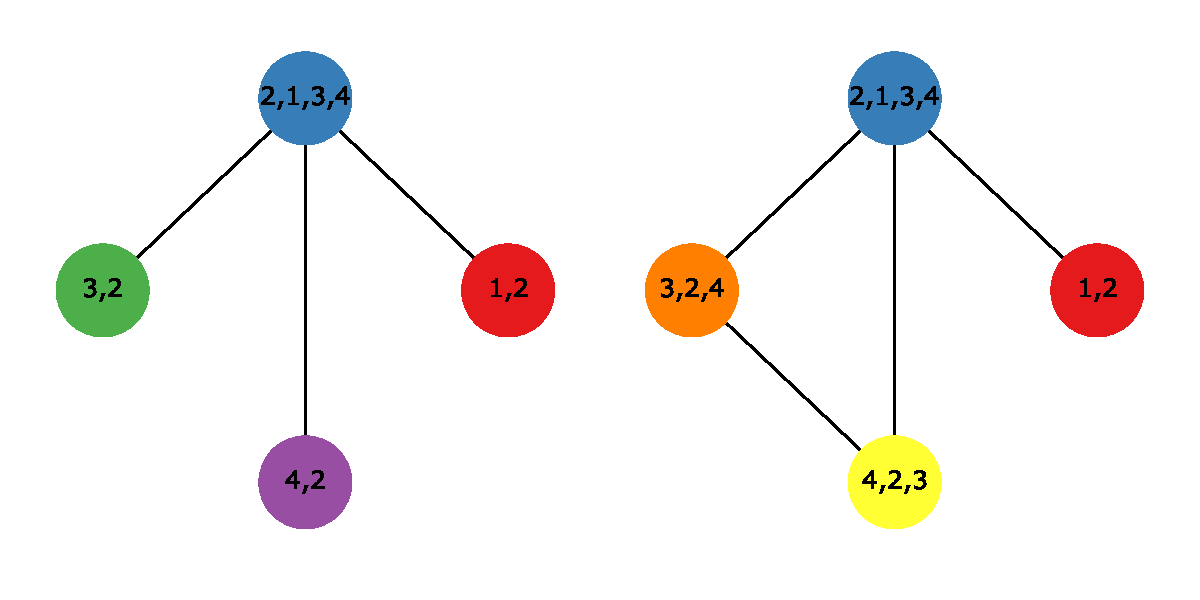
\includegraphics[width=\linewidth]{assets/figures/wl_examples/wl_iteration_1_stage_0_recolored}}
  \caption{$h=1$: After relabeling}
  \end{subfigure}
  \begin{subfigure}[t]{0.49\linewidth}
  {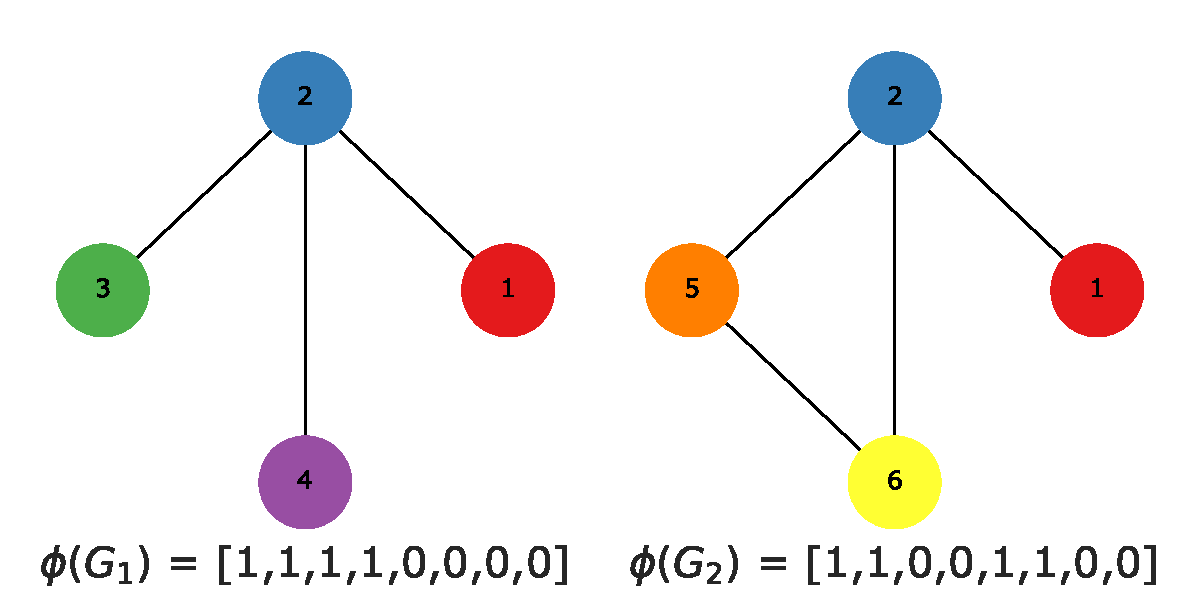
\includegraphics[width=\linewidth]{assets/figures/wl_examples/wl_iteration_1_stage_1_compressed.pdf}}
  \caption{$h=1$: After label compression}
  \end{subfigure}
\begin{subfigure}[t]{0.49\linewidth}
{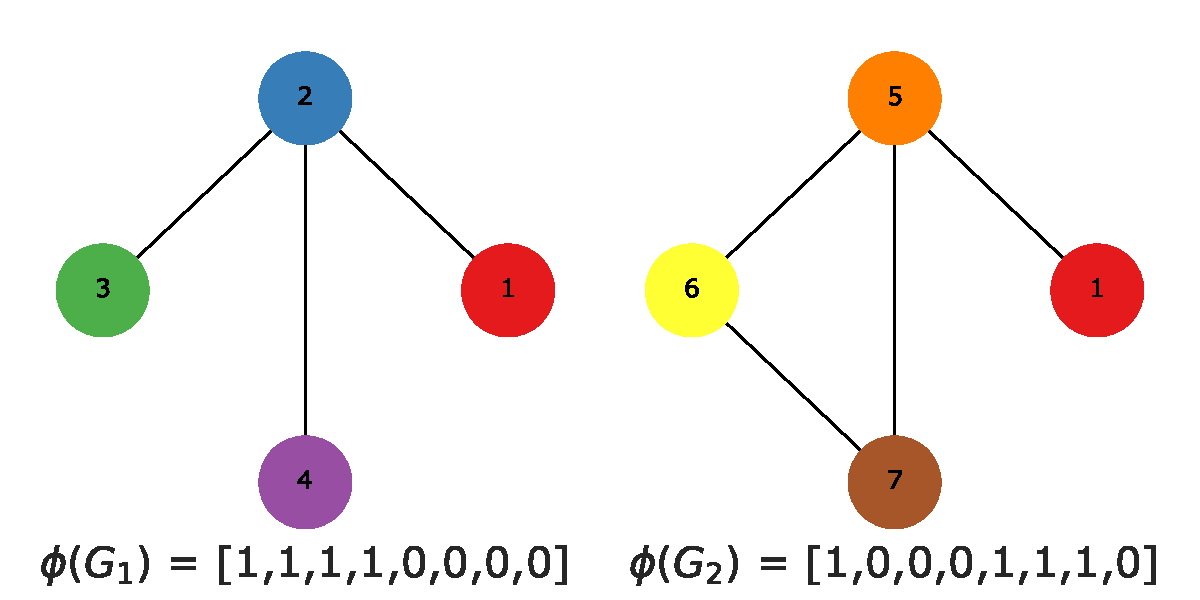
\includegraphics[width=\linewidth]{assets/figures/wl_examples/wl_iteration_2_stage_1_compressed.pdf}}
\caption{$h=2$: After label compression}
\end{subfigure}
	\caption[Example: Weisfeiler Lehman iteration]{Weisfeiler Lehman algorithm example. This examples shows one WL iteration with two graphs, $G_1$ and $G_2$. The initial graphs are shown in \textbf{(a)}. The first step of a WL iteration is relabeling the graph vertices by concatenating each node label with its sorted neighborhood labels. The finished relabeled graph is shown in \textbf{(b)}. As an extension to the plain Weisfeiler-Lehman algorithm, we also show the label compression step where the long labels, consisting of the node label and its neighborhood labels, get compressed into a smaller label by assigning each unique label a new number. Same multi-label labels in different graphs get the same new label. The result of this step is shown in \textbf{(c)}. Under \textbf{(a)},  \textbf{(b)} and \textbf{(d)} we also added the feature maps $\phi(G)$ for both graphs. Each entry in the vector corresponds to a label. If a vector entry is 1, the corresponding label is present in the graph. The inner product on the vectors of the graphs is the value of the Weisfeiler-Lehman graph kernel for these two graphs.
  In this case, the similarity before the iteration would be $\langle \phi(G_1), \phi(G_2) \rangle = \langle [1, 1, 1, 1, 0, 0, 0, 0], [1, 1, 1, 1, 0, 0, 0, 0] \rangle = 4$. After the relabeling, the value of the inner product is $2$.
  Before doing the WL iteration, the inner product on the feature maps simply returns the number of common labels. After the first iteration, the neighborhood of each node and therefor the structure of the graph is also reflected in the feature map - resulting in a lower similarity in out example.
  Notice that before the relabeling, ie. in \textbf{(a)}, the labels for the left-most node was the same for both graphs. After the first iterations, in \textbf{(b)} and \textbf{(c)}, they get different colors.
  The same happens for the top-most node: after the second iteration, in \textbf{(d)}, the labels are also different since in iteration $h=2$ not only the immediate neighborhood has to be the same for a match, also the neighborhood of its neighborhood.}
	\label{fig:wl_example}
\end{figure}

\labelsection{Graph Kernel Based Text Classification}{subsec:graph_kernel_based_text_classification}
The idea of converting the text classification task into a graph classification task has been explored before.
In this section, we will briefly recap the history of this approach by explaining several papers related to our work.
While most of the graph classification approaches are used in context where graphs are the default representation of the data at hand, here we mostly explore papers which also derive graphs from existing text.

\labelsubsection{Related Work}{subsection:related_work}

\paragraph{``Shortest-Path Graph Kernels for Document Similarity" \cite{Nikolentzos2017a}}
The most similar and recent work to our approach that we found was \cite{Nikolentzos2017a}. In this work, the authors first create co-occurrence graphs out of the text. Next, they create the gram matrix for the graphs with their own graph kernel and use a SVM to classify them.

Their graph kernel is a combination of two sub-kernels:
\begin{enumerate}
    \item{\textit{Simple label matching}: the number of matching node labels are compared between the two graphs}
    \item{\textit{Shortest path}: generate a shortest-path graph, then compare the edges}
\end{enumerate}
Note that the simple label matching sub-kernel does not take the structure into account, while the second sub-kernel actually uses both.
Both sub-kernels return a number which is added to produce the final value of the kernel.

The shortest path sub-kernel works as follows:
\begin{enumerate}
    \item{Generate shortest-path graphs for the two given graphs: The shortest path graph of a given graph has the same nodes.
    The edges are added by calculating the shortest paths between all pairs of nodes in the original graph. An edge is added between two nodes in the shortest path graph if the shortest path length between these nodes in the original graph is below a given parameter $d$. The edge also gets a weight assigned, which is $\frac{1}{d}$}
    \item{Count the number of same edges in the both graphs: when two edges are the same, add the product of their edge weights to the similarity}
\end{enumerate}

One thing to note about this work is that they used a combined kernel, yet they did not evaluate the performance or importance of each sub-kernel for the classification, ie. they did not report results for each sub-kernel.
The simple-set-matching algorithm by itself has a high performance and most likely has the highest contribution to the classification results. We performed simple checks on the same datasets with only the simple-set-matching sub-kernel without their proposed shortest-path extension and got similar scores.
A more thorougher analysis would be helpful to get a better insight.

That said, this approach is quite similar to ours. In their approach, they also convert the texts into graphs and then classify the graphs. One difference to our approach is, besides that we use different kernels and more datasets, that we evaluate the performance of concept maps instead of only co-occurrence graphs.

\paragraph{``Text Categorization as a Graph Classification Problem" \cite{Rousseau2015a}}
In this paper, the authors generate co-occurrence graphs out of different text classification datasets.
To classify the graphs, they introduce their own graph kernel which is also an instance of the aforementioned kernels that count the number of occurrences of sub-structures.
In this case, the sub-structures this kernel counts are frequent subgraphs, ie. subgraphs that occur frequently in the graphs of the dataset.
To get a set of most-frequent subgraphs in the dataset, they develop their own approach, using depth-first search and a labeling function for graphs that enables finding frequent subgraphs efficiently.
After extracting the sub-graphs from the dataset this way, they only retain subgraphs which occur more often in the dataset than some defined parameter, the support value.
This significantly reduces the number of considered sub-graphs since most subgraphs occur quite infrequently.
This extension is indeed needed since the number of possible sub-graphs grows super-linear with the number of nodes/edges and can render the subsequent counting of the sub-graphs in the dataset infeasible.
Also, considering all possible subgraphs in all graphs in the dataset would not only require significant computational resources but would also result in sparse feature vectors since most sub-graphs occur infrequently.
This, in turn, would harden the classifier training problem.

As another measure to lower the runtime complexity of their algorithm, they also first extract the main core of each co-occurrence graph and only extract sub-graphs from them, not from the whole graphs.
A $k$-core is a subgraph $G_k$ of graph $G$ where all vertices have a degree greater or equal to $k$. The main core of a graph is the $k$-core with the highest possible $k$.
Thus the main core is the most connected subgraph of graph $G$, which includes only the most ``important" vertices and their edges to each other.

So, after extracting the main-core of each co-occurrence graph and determining the set of most-frequent sub-graphs in the dataset, they count the occurrences of the most-frequent sub-graphs for each graph in the dataset.
This results in feature maps $\phi_i$ which contain the counts of each most-frequent sub-graph per co-occurrence graph.
These feature vectors together with the labels are then used to train a SVM and are used to subsequently predict new instances by creating their feature maps and then predicting the label with this trained SVM.

The authors evaluated the classification performance of their approach on several datasets, namely the \textit{WebKB} corpus, a subset of the \textit{reuters-21578} corpus (named R8), the \textit{ling-spam} dataset and a corpus of \textit{Amazon reviews}.
In our work, we also use these and other datasets. In later sections, we will introduce then more thoroughly.

In the paper, the authors argue that only retaining the main-core does not greatly damage the classification performance, yet it significantly reduces the compute time.
They also stress the importance of choosing an adequate support value for the sub-graph mining, mentioning the trade-off between performance and considered features. The process of choosing an adequate support value can be done unsupervised and gets treated similar to hyperparameter tuning of, for example, SVM hyperparameters.

This paper is quite similar to our approach since it also poses the text classification task as a graph classification task. Yet, they consider only one type of graph, the co-occurrence graph.
Also, they do not evaluate the effect of combining text- and graph features.
That said, they provide interesting comparisons of text- and graph based approaches, pointing out the similarity of n-grams with the relationships which are captured in co-occurrence graphs.

\paragraph{``Concept Graph Preserving Semantic Relationship for Biomedical Text Categorization" \cite{Gulrandhe2015}}
The paper explores also explores the usefulness of using automatically generated concept graphs for text classification.
They first extract a concept graph for each of the articles in a medical dataset. Constructing the concept graph was done by extracting noun phrases with a \textit{Part-of-Speech} short \textit{POS}, tagger.
Next, these extracted noun phrases are then looked up in the medical database called \textit{UMLS}. When a noun phrase is found in this database, it becomes a node for the concept graph that is generated from th text. Other noun phrases are ignored.
This additional filtering is done to find important concepts in a controlled vocabulary which can be further enriched by relationships which are also stored in the \textit{UMLS} database.
The relationships between concepts in the \textit{UMLS} database are semantic, eg. whether two concepts are synonyms for each other.
These relationships are then used as the edges between the concepts in the generated concept graph.
In the next step, they gather node specific metrics, eg. the frequency of concepts in the underlying text, and sum them up to retrieve a weight $w_v$ for each node $v$.
Next, they obtain edge weights for each edge $e = (v, v')$ between two nodes $v$ and $v'$ by adding up the weights of both nodes, ie. $w_e = d_v + d_{v'}$.
Then they remove edges which have a weight below some given threshold.
After generating the concept graphs in this manner, the authors use a simple edge matching kernel to calculate the gram matrix for concept graphs.
The kernel they use is similar to the graph kernel we introduced before, namely the \textit{Simple Non-Structural Graph Kernel}: instead of counting the number of common nodes, as in our example, they instead match the edges.
As a final step, they train a kernelized \textit{SVM} and a kernelized \textit{k-Nearest-Neighbor} classifier with the gram matrix for the concept graphs and the labels as input.

Unfortunately, the authors do not report their classification scores or provide the means to obtain the used dataset. 
Therefore an analysis of the claim is hardly testable that their approach shows statistically significant improvement over conventional, text-based approaches.
That said, their approach is quite similar to our approach: they also use noun phrases extracted from a text to subsequently train a kernelized \textit{SVM}.
Yet, while they use semantic relationships obtained from a database as edges, we obtain the edges directly from the text.
Also, we use different kernels to leverage multiple aspects of the structure and content of the concept maps. The authors, on the other hand, only evaluate one kernel capitalizing on the edges between concepts.

\paragraph{``Text classification using Semantic Information and Graph Kernels" \cite{Gaspar2011}}
In this paper, the text classification task is also converted into a graph classification task.
The authors create a graph of the underlying text by extracting so-called \underline{D}iscourse \underline{R}epresentation \underline{S}tructures, or DRS, which capture the semantic relationships in the sentences of the underlying text.
A DRS consists of two parts, namely a set discourse referents, or entities, and conditions on these entities.
The example given in the paper constructs the DRS for the sentence ``He throws the ball", which results in the DRS with the entities $\{\text{He}, \text{ball}, \text{throws}\}$ which get renamed to $\{x1, x2, x3\}$.
The conditions of the DRS then define the meaning or relationship between entities.
For the mentioned example, the DRS conditions are $\{\text{male}(x1), \text{ball}(x2), \text{throws}(x3), \text{event}(x3), \text{agent}(x3, x1), \text{patient}(x3, x2)\}$.
To construct a graph from the extracted DRSs, the entities become vertices and the conditions become edges between them.
A unary condition on a vertex, for instance $\text{male}(x1)$, becomes a loop for the node $x1$.
Conditions on two entities become directed edges, going from the entity of the first argument to the second condition argument, for example the condition $\text{agent}(x3, x1)$ creates a node from $x3$ to $x1$.
This results in a graph which captures the semantic relationship between the entities of the underlying graph.
Note that edge node labels, or entities, are not as important as the edges , or conditions, between them.
This is accounted for in the kernel the authors use in the next step.
Also note, that the process of creating a DRS graph for a given text is independent of other texts and can easily be parallized.

After constructing DRS graphs for all texts in the dataset, the authors use a variant of a random-walk kernel, customized to capture the importance of the edges instead of the nodes.
In the plain random-walk kernel, random walks are done on the two graphs, $G$ and $G'$ and the counts of equal random walks are counted, resulting in a measure of similarity between these two graphs. The higher the count of equal random walks, the higher the similarity.
The equality of two walks is determined by comparing the labels of the visited nodes.
In the case of DRS graphs, this would not yield a good kernel since the labels of the nodes are placeholders, ie. two vertices with the same label, for example $x1$, can correspond to totally different entities.
So, the standard definition of walk equality can not be used in the case of DRS graphs.
Instead, the authors introduce an approach which, for a given node $v_1$ of graph $G$, returns an ``equal" node $v_2$ in graph $G'$ that has similar edge \textbf{labels}.
This enables the random-walk graph kernel to ``merge" nodes with different node labels, that is placeholder like $x1$, on the two graphs, thus enabling random walks with meaningful node equality in the case of the DRS graphs.
After extracting the gram matrix of the DRS graphs with this extended random-walk graph kernel, the authors then use a SVM to evaluate their approach on the \textit{reuters-21578} dataset.
They use only a subset of 50 texts in the five most frequent classes of the dataset as their corpus. Then they create the DRS graphs for these texts and randomly select 25 of each class to create a gram matrix.
This gram matrix then gets used to train a one-versus-one SVM classifier. So, they do binary classification and present the results of the performance of the pairs of the 5 classes they considered.
The authors explain the reason for this small number of considered documents and classes by mentioning the runtime complexity of their approach, most notably the runtime complexity of the random-walk kernel.
They also acknowledge that they do not provide baseline results or comparisons between different approaches to text-classification or results with other graph kernels.

That said, this work is also similar to our approach in the sense that they also use graphs representations of texts to classify.

\paragraph{``Deep Graph Kernels" \cite{Yanardag2015}}
In this paper, the authors introduce an extension for existing kernels for which the explicit feature map $\phi$ can be calculated.
When calculating the kernel
\begin{equation*}
k(G, G') = \phi^T(G) \cdot \phi(G')
\end{equation*}
they add a weighting matrix $M$
\begin{equation*}
k(G, G') = \phi^T(G) \cdot M \cdot \phi(G')
\end{equation*}

The intuition here is that each vector entry of $\phi(G)$ corresponds to the count of some substructure of $G$ and that these substructures are not independent of each other, ie. they can be similar to each other.
Yet when calculating the plain kernel only exact matches of substructures in the two graphs are considered.
For instance, suppose substructure $g_1$ is similar to another substructure $g_2$ and substructure $g_1$ is only present in $G$ and not in $G'$, conversely substructure $g_2$ is only present in $G'$ and not in $G$.
Suppose some kernel $k$ would construct $\phi_k(G)$ by counting the occurrences of $g_1$ and $g_2$, so $\phi_k(G) = (n_{g_1}(G), n_{g_2}(G))$ where $n_{g_i}(G)$ counts the occurrence of substructure $g_i$ in $G$.
In the above example, $\phi_k(G_1) = (1, 0)$ and $\phi_k(G_2) = (0, 1)$. When calculating $k(G, G') = \phi_k^T(G) \cdot \phi_k(G') $ the similarity under the kernel would equal 0, therefore ignoring the similarity of substructure $g_1$ and $g_2$.
The proposed extension to the kernel aims to address this issue by using embeddings for the substructures to identify the similarity of substructures and then allowing ``partial" instead of only exact matches.
In the above example, the new $\phi_{new}(G)$ would not be $(1, 0)$ but $(1, i)$ and $\phi_{new}(G') = (i, 1)$ with some $i > 0$.
In our example, the aforementioned matrix $M$ would be
\begin{align*}
M = \begin{bmatrix}
1 & i \\
i & 1
\end{bmatrix}
\end{align*}

In this case, when calculating the kernel for these two graphs, the similarity would be $(1, 0)^T \cdot M \cdot (0, 1) = (1, 0)^T \cdot (i, 1) = i$ instead of $(0, 1)^T \cdot (1, 0) = 0$.
So, the augmented kernel between these graphs would actually capture the similarity of substructures instead of only using exact matches of them.

The authors then introduce two ways to create the matrix $M$ for a kernel, namely by creating it by hand using a measure of similarity between the substructures or by learning the embeddings with an approach similar to the \textit{word2vec} algorithm.
In both cases, the matrix $M$ aims to encode the similarities of the substructures.

The authors report an improvement of classification scores for several real-world datasets, comparing the scores of the plain version of a kernel with their augmented version.

\labelsubsection{Summary}{subsection:related_work_summary}
As we see, several graph representations for text have been studied in the context of text classification.
Yet, our approach differs in some crucial ways from the previous work, namely that (1) we capitalize on concept maps, a graph representation which is known for its summarization capabilities, resulting in smaller graphs. Also (2) we explicitly compare our results with conventional text-based approaches that achieve state-of-the-art performance.
And while others mainly used graph kernels which are not able to be easily combined with text-based approaches, we (3) capitalize on graph kernels where the explicit feature map $\phi$ can be generated.
This, in turn, enables us to explore an approach where we combine conventional text features, eg. \textit{BoW}, with features obtained from these graph kernels.